\chapter{Quantenmechanik}

\section{Grundlagen}

\begin{enumerate}[i)]
	\item \textbf{Wellenfunktion} $ \Psi(\vec{r}) $ $ \qquad $ mit $ \vec{r} $ der \textbf{Ortsdarstellung}
	\begin{equation*}
	P = \int_{V} \left|\Psi ( \vec{r})\right|^2 \dd \vec{r} \quad \tx{Wahrscheinlichkeit} \qquad \quad \int_{V} \left|\Psi(\vec{r})\right|^2 \dd \vec{r} = 1 \quad \tx{Normierungsbedingung}
	\end{equation*}
	\item \textbf{Operatoren} $ \hat{O} $
	\begin{equation*}
	\hat{O} \Psi(\vec{r}) = \Psi'(\vec{r})
	\end{equation*}
	Korrespondenzprinzip
	\begin{align*}
	\vec{r} &= \hat{\vec{r}} \qquad \hat{\vec{r}} \Psi(\vec{r}) = \Psi'(\vec{r}) = \vec{r} \Psi(\vec{r}) \qquad \quad ; \quad \, \rmbox{\hat{x} \Psi(x) = x \Psi(x) = \Psi'(x)} \\
	\vec{p} &= \hat{\vec{p}} \qquad \hat{\vec{p}} \Psi(\vec{r}) = \Psi'(\vec{r}) = - i \hbar \vabla \Psi(\vec{r}) \quad ; \quad \rmbox{\hat{p}_{x} \Psi(x) = - i \hbar \prd{}{x} \Psi(x) = \Psi'(x) }
	\end{align*}
	$ \hat{\ham} = $ Hamiltonian oder Hamilton-Operator. $ \hat{\ham} = \hat{\ham}(\hat{\vec{r}} , \hat{\vec{p}}) $
	\begin{equation*}
	\hat{\ham} = \frac{\hat{p^2}}{2m} + V(\vec{r}) = - \frac{\hbar^2}{2m} \vabla^2 + V(\vec{r})
	\end{equation*}
	\item \textbf{Zeitabhängige Schrödinger Gleichung}
	\begin{equation*}
	\rmbox{i\hbar \prt{}{t} \Psi(\vec{r}, t) = \hat{\ham}  \Psi(\vec{r}, t)}
	\end{equation*}
	Die klassische Energie sieht so aus:
	\begin{equation*}
	E = \frac{p^2}{2m} + V(\vec{r})
	\end{equation*}
	In der QM dann folgendermaßen:
	\begin{equation*}
	\hat{\ham} = \frac{\hat{p}^2}{2m} + V(\vec{r})
	\end{equation*}
	Die \textbf{Zeitunabhängige Schrödinger Gleichung} sieht wie folgt aus:
	\begin{equation*}
	\rmbox{\hat{\ham} \Psi(\vec{r}) = E \Psi(\vec{r})}
	\end{equation*}
	Diese Gleichung ist eine Eingenwertgleichung. Der Hamilton Operator liefert also den Energie-Eingenwert $ E $ und die Eigenzustände $ \Psi(\vec{r}) $.
	
	\subsection*{Stationäre Zustände}
	
	Jeder messbaren Physikalische Größe ist ein Operator $ \hat{O} $ zugeordnet. Bei einer physikalischen Messung wir der \textbf{Erwartungswert} gemessen: $ \langle \hat{O} \rangle = \langle \Psi | \hat{O} | \Psi \rangle $.
	\begin{equation*}
	\langle \hat{O} \rangle = \langle \Psi(\vec{r}) | \hat{O} | \Psi(\vec{r}) \rangle = \int \Psi^*(\vec{r}) \ \ub{ \hat{O} \ \ \Psi(\vec{r}) }_{\Psi'(\vec{r})} \dd \vec{r}
	\end{equation*}
	\begin{equation*}
	\langle \hat{O}(t) \rangle = \langle \Psi(\vec{r},t) | \hat{O} | \Psi(\vec{r},t) \rangle = \int \Psi^*(\vec{r},t) \hat{O} \Psi(\vec{r},t) \dd \vec{r}
	\end{equation*}
	Diese Gleichung können wir wie folgt umformen:
	\begin{equation*}
	\Psi(\vec{r},t) = \Psi(\vec{r},t = 0) \ub{e^{- \nicefrac{i E t}{\hbar}}}_{\tx{Phasenfaktor}}
	\end{equation*}
	\begin{align*}
	\langle \hat{O} \rangle &= \int \Psi^*(\vec{r}, t = 0) \cancel{e^{\nicefrac{i E t}{\hbar}}} \hat{O} \Psi(\vec{r}, t = 0) \cancel{e^{- \nicefrac{i E t}{\hbar}}} \dd \vec{r} \\
	&= \int \Psi^*(\vec{r}, t = 0) \hat{O} \Psi(\vec{r} , t = 0) \dd \vec{r} \overset{*}{=} \langle \hat{O}(t = 0) \rangle
	\end{align*}
	$ *: $ wenn $ \hat{O} $ nicht Zeitabhängig ist.\\[5pt]
	\textbf{Stationäre Zustände}
	\begin{equation*}
	i \hbar \prt{}{t} \Psi(\vec{r}, t) = \hat{\ham} \Psi(\vec{r}, t) \qquad \tx{mit} \qquad \Psi(\vec{r},t) e^{- \nicefrac{i E t}{\hbar}} \Psi(\vec{r} ,t = 0)
	\end{equation*}
	\begin{equation*}
	\frac{\partial \Psi}{\Psi} = - i \frac{\hat{\ham}}{\hbar} \partial t
	\end{equation*}
	Lösung der DGL mittels Variablen-Trennung
	\begin{equation*}
	\ln\left[\frac{\Psi(\vec{r},t)}{\Psi(\vec{r}, t = 0)}\right] = - \frac{i \hat{\ham} t}{\hbar} \quad \Rightarrow \quad \Psi(\vec{r}, t) = e^{- \nicefrac{i \hat{\ham} t}{\hbar}} \Psi(\vec{r}, t = 0)
	\end{equation*}
	\begin{equation*}
	\hat{\ham} \Psi(\vec{r} , t = 0) = E \Psi(\vec{r}, t = 0)
	\end{equation*}
	Taylor Entwicklung:
	\begin{equation*}
	e^{x} = e^{- \nicefrac{i \hat{\ham} t}{\hbar}} = a \left(\hat{\ham}\right)^0 + b \left(\hat{\ham}\right)^1 + c \left(\hat{\ham}\right)^2 + \dots
	\end{equation*}
	\begin{align*}
	e^{- \nicefrac{i \hat{\ham} t}{\hbar}} \Psi(\vec{r}, t = 0)&= a \Psi(\vec{r}, t = 0) + b \hat{\ham} \Psi(\vec{r}, t = 0) + c \hat{\ham} \cdot \hat{\ham} \Psi(\vec{r}, t = 0) + \dots \\
	&= a \Psi(\vec{r}, t = 0) + b E \Psi(\vec{r}, t = 0) + c E^2 \Psi(\vec{r}, t = 0) + \dots \\
	&= (a + bE + c E^2 + \dots) \cdot \Psi(\vec{r}, t = 0) \\
	&= e^{- \nicefrac{i E t}{\hbar}} \Psi(\vec{r}, t = 0)
	\end{align*}
	\lcom{Wir können einen Operator in der $ e $-Funktion schreiben, da diese mit der Taylorentwicklung als Reihe entwickelt werden kann.}
	\item \textbf{Spin} (Elektronen)
	\begin{enumerate}[$ \Rightarrow $]
		\item Wasserstoffatom (Stern-Gerlach)
		\item Helium (Pauli Prinzip)
	\end{enumerate}
	\newpage
	\item \textbf{Quantensysteme}
	\begin{itemize}
		\item Freies Teilchen, Potentialstufe (Tunneln)
		\item Harmonischer Oszillator $ \Rightarrow $ Molekülphysik
		\item Coulomb Potential $ \Rightarrow $ Wasserstoffatom
	\end{itemize}
	\begin{figure}[ht]
		\centering
		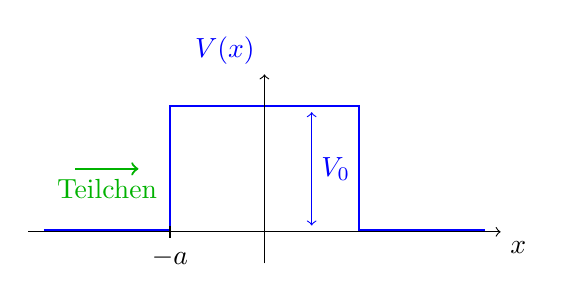
\begin{tikzpicture}[scale=0.8]
		\draw[thick,blue] (-3.5,.025) -| (-1.5,2) -- (1.5,2) |- (3.5,.025);
		\draw[thick,black!30!green,->] (-3,1) -- node[below] {Teilchen} ++(1,0);
		\draw[->] (-3.75,0) -- (3.75,0) node[anchor=north west] {$ x $};
		\draw[->] (0,-0.5) -- (0,2.5) node[anchor=south east] {\color{blue}$ V(x) $};
		\draw (-1.5,.1) -- ++(0,-.2) node[below] {$ -a $};
%		\draw (1.5,.1) -- ++(0,-.2) node[below] {$ +a $};
%		\node[draw=black,circle, minimum size=.8cm,red] at (-2.5,-1) {I};
%		\node[draw=black,circle, minimum size=.8cm,red] at (0,-1) {II};
%		\node[draw=black,circle, minimum size=.8cm,red] at (2.5,-1) {III};
		\draw[<->,blue] (.75,.1) -- node[right] {$ V_0 $} ++(0,1.8); 
		\end{tikzpicture}
		\label{Potentialbarriere}
		\caption{Darstellung einer Potentialbarriere. Beispiel für den Tunneleffekt eines hindurchfliegenden Teilchens, das eigentlich weniger Energie hat als klassisch nötig wäre um die Barriere zu überwinden. Dieses Bild wurde mit dem \LaTeX Paket Tikz erstellt.}
	\end{figure}
	\FloatBarrier
	\item \textbf{Kommutatoren}
	\begin{align*}
	\hat{x}&: \vec{p} = \vec{p}_x \qquad \qquad \left[\hat{x}, \hat{p}\right] = \hat{x} \hat{p} - \hat{p} \hat{x} \\
	\hat{A}; \hat{B}&: \qquad \qquad \qquad \ \left[\hat{A}, \hat{B}\right] = \hat{A} \hat{B} - \hat{B} \hat{A}
	\end{align*}
	Wellenfunktion $ \Psi(x) \qquad \qquad \left[\hat{x}, \hat{p}\right] \Psi(x) = \Psi'(x) $
	\begin{equation*}
	\left[\hat{x}, \hat{p}\right] = \hat{x} \hat{p} - \hat{p} \hat{x} = x \left(- i \hbar \prd{}{x}\right) - \left(- i \hbar \prd{}{x}\right) x
	\end{equation*}
	\begin{align*}
	\left[\hat{x}, \hat{p}\right] \Psi(x) &= \left\{ x \left(- i \hbar \prd{}{x}\right) - \left(- i \hbar \prd{}{x}\right) x \right\} \Psi(x) \\
	&= x \left(- i \hbar \prd{}{x} \Psi(x) \right) - \left(- i \hbar \prd{}{x}\right) x \Psi(x) \\
	&= - i \hbar x \prd{\Psi}{x} + i \hbar \prd{}{x} ( x \Psi(x)) \\
	&= \cancel{ - i \hbar x \prd{\Psi}{x}} \cancel{+ i \hbar x \prd{\Psi}{x}} + i \hbar \Psi(x) \ub{\prd{x}{x}}_{=1} \\
	&= i \hbar \Psi(x) = \Psi'(x)
	\end{align*}
	\begin{equation*}
	\rmbox{\left[\hat{x}, \hat{p}\right] = i \hbar} \quad \Rightarrow \quad \tx{die zwei Operatore vertauschen nicht !!!}
	\end{equation*}
	
	\subsection*{Eigenschaft Kommutator}
	
	$ \hat{A} $; $ \hat{B} $
	\begin{equation*}
	\Delta A \cdot \Delta B \ge \frac{1}{2} \left| \langle \left[\hat{A}, \hat{B}\right] \rangle \right|
	\end{equation*}
	$ \left[\hat{A}, \hat{B}\right] $ Operator $ \Rightarrow $
	\begin{align*}
	\langle \left[\hat{A}, \hat{B}\right] \rangle &= \langle \hat{A} \hat{B} - \hat{B} \hat{A} \rangle \\
	&= \langle \Psi | \hat{A} \hat{B} - \hat{B} \hat{A} | \Psi \rangle \\
	&= \int \Psi^* \left(\hat{A} \hat{B} - \hat{B} \hat{A}\right) \Psi \dd \vec{r}
	\end{align*}
	$ \Delta A $, $ \Delta B $ Standardabweichung
	\begin{equation*}
	\sigma_x = P(x) \quad \sigma_x = \left[ \int (x - \mu)^2 P(x) \dd x \right]^{1/2}  \qquad \mu = \int x P(x) \dd x
	\end{equation*}
	
	% T Gaußglocke
	
	\begin{figure}
		\centering
		\begin{tikzpicture}
			\draw[->] (0,-0.2) -- (0,2.5) node[anchor=south east] {$ P(x) $};
			\draw[->] (-0.2,0) -- (7,0) node[anchor=north west] {$ x $};
			\draw[domain=0:7, samples=80, thick] plot (\x, {2*exp(-(\x - 3.5)^(2)*0.6});
			\coordinate (o) at (3.5,1);
			\coordinate (d) at (1.1,0);
			\draw[ultra thick, <->, blue, arrows = {Stealth}-{Stealth}] ($ (o) + (d) $) -- ($ (o) - (d) $);
		\end{tikzpicture}
		\label{Gausverteilung}
		\caption{Die Wahrscheinlichkeitsverteilung einer Gaußkurve. Der Pfeil soll die Standartabweichung darstellen. Dieses Bild wurde mit dem \LaTeX Paket Tikz erstellt.}
	\end{figure}
	
	$ \hat{A} = \hat{x} $, $ \hat{B} = \hat{p} $. $ \left[\hat{x}, \hat{p}\right] = i \hbar $
	\begin{equation*}
	\Delta A \cdot \Delta B \ge \frac{1}{2} \left| \langle \left[\hat{A}, \hat{B}\right] \rangle \right|
	\end{equation*}
	\begin{equation*}
	\Delta x \cdot \Delta p \ge \frac{1}{2} \left| i \hbar \right| = \frac{\hbar}{2}
	\end{equation*}	
\end{enumerate}

\subsection*{Morgen:}

Operatoren die vertauschen: Drehimpulsoperator $ \vec{l} $ mit den Komponenten $ l_x, l_y, l_z $ und $ l^2 $. Es gilt $ \left[l^2, l_z\right] = 0 $
\begin{equation*}
\Delta l^2 \cdot \Delta l_z \ge 0
\end{equation*}
Man kann also Zustände finden, bei denen $ \Delta l^2 = 0 $; $ \Delta l_z = 0 $ sind. Diese Zustände können im Prinzip existieren und verletzen die Unschärferelation nicht! Diese Zustände sind dann gleichzeitig Eigenzustände von $ l^2 $ und $ l_z $.

\subsubsection*{Exkurs: Varianz und Standardabweichung in der Quantenmechanik}

Wellenfunktion $ \Psi(x) $ mit Wahrscheinlichkeit $ P(x) = |\Psi(x)|^2 $
\begin{align*}
\mu &= \int x P(x) \dd x = \int x | \Psi(x) | ^2 \dd x \\
\sigma   &= \int x^2 P(x) \dd x = \int x^2 | \Psi(x) | ^2 \dd x
\end{align*}
Die Varianz ist definiert als:
\begin{align*}
\sigma^2 = \int (x - \mu)^2 P(x) \dd x &= \int (x^2 + \mu^2 - 2 \mu x) P(x) \dd x \\
&= \int x^2 P(x) \dd x + \mu^2 \int P(x) \dd x - 2 \mu \int x P(x) \dd x\\
&= \int x^2 P(x) \dd x + \mu^2 - 2 \mu \mu = \int x^2 P(x) \dd x - \mu^2 \\
&= \langle x ^2 \rangle - \langle x \rangle ^2
\end{align*}

% 26.04.19

\subsection*{Programm Heute}

\begin{itemize}
	\item Drehimpulsoperator
	\item Kugelflächenfunktionen (Wasserstoffatom)
	\item Vektormodell (klassische Darstellung)\\
	\lcom{Macht es leichter z.B. die Wechselwirkung zwischen Drehimpulsoperator und Magnetfeld zu verstehen. Dieses klassische Modell macht voraussagen über die QM.}
	\item Experimente (Spektrum des Wasserstoffatoms)
	\item Schrödinger Gleichung des Wasserstoffatoms
\end{itemize}

\section{Drehimpulsoperator}


\begin{minipage}{.5\linewidth}
	\begin{equation*}
	\vec{l} = \vec{r} \times \vec{p} = \vec{r} \times m \vec{v}
	\end{equation*}
	\begin{align*}
	\vec{r} & \Rightarrow \hat{\vec{r}} = \vec{r} \\
	\vec{p} & \Rightarrow \hat{ \vec{p}} = - i \hbar \vabla \\
	\vec{l} & \Rightarrow \hat{\vec{l}} = \vec{r} \times (- i \hbar \vabla) = - i \hbar \vec{r} \times \vabla
	\end{align*}
\end{minipage}%
\begin{minipage}{.5\linewidth}
	\flushright
	%t1:
	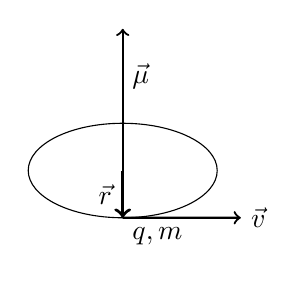
\begin{tikzpicture}[scale=.6]
		\draw[thick, ->] (0,0) -- (0,3);
		\draw (0,0) ellipse(2cm and 1cm);
		\coordinate (a) at (0,-1);
		\node[right] at (0,2) {$\vec{\mu}$};
		\node[anchor=north west] at (a) {$q,m$};
		\draw[very thick,->] (0,0) -- node[left] {$ \vec{r} $} (a);
		\draw[thick,->] (a) -- (2.5,-1) node[right] {$\vec{v}$};
	\end{tikzpicture}
\end{minipage}%
\\[5pt]
\begin{equation*}
\hat{\vec{l}} = - i \hbar \begin{vmatrix}
\vec{u}_x & \vec{u}_y & \vec{u}_x \\
x & y & z \\
\prt{}{x} & \prt{}{y} & \prt{}{z}
\end{vmatrix} = - i \hbar
\end{equation*}

%t2
\begin{tikzpicture}[scale=0.6]
	\draw[->] (0,0) -- (3,0) node[anchor=north west] {$ y $};
	\draw[->] (0,0) -- (0,3) node[anchor=south east] {$ z $};
	\draw[->] (0,0) -- (-2,-2) node[anchor=north east] {$ x $};
	\draw[red, thick, ->] (0.5,0.2) -- node[above] {$ \vec{u_y} $} ++(1,0);
	\draw[red, thick, ->] (-0.2,0.5) -- node[left] {$ \vec{u_z} $} ++(0,1);
	\draw[red, thick, ->] (0.0,-0.3) -- node[anchor=north west] {$ \vec{u_x} $} ++(-0.8,-0.8);
\end{tikzpicture}

\begin{align*}
l_x &= - i \hbar \left\{ y \prt{}{z} - z \prt{}{y} \right\} \\
l_y &= - i \hbar \left\{ z \prt{}{x} - x \prt{}{z} \right\} \\
l_z &= - i \hbar \left\{ x \prt{}{y} - y \prt{}{x} \right\}
\end{align*}
\begin{align*}
\left[l_x, l_y\right] = l_x l_y - l_y l_x \neq 0
\end{align*}

\subsection*{Vertauschungsregeln}

\begin{align*}
\left[l_x, l_y\right] &= i \hbar l_z \\
\left[l_y, l_z\right] &= i \hbar l_x \\
\left[l_z, l_x\right] &= i \hbar l_y
\end{align*}
Das Betragsquadrat berechnet sich wie folgt: $ l^2 = l_x^2 + l_y^2 l_z^2 $

\subsection*{Vertauschungregeln}

\begin{equation*}
\left[l^2, l_x\right] = \left[l^2, l_y\right] = \left[l^2, l_z\right] = 0
\end{equation*}
Wir werden bevorzugt $ l_z $ verwenden.\\[10pt]
\noindent
Die Eigenzustände von $ l_z $
\begin{equation*}
l_z = - i \hbar \left\{ x \prt{}{y} - y \prt{}{x} \right\} = - i \hbar \prt{}{\varphi}
\end{equation*}

%T3

\noindent
$ l_z \Rightarrow $ Drehung um die $ z $-Achse\\[10pt]
\noindent
Wir suchen die Operatoren $ \Phi(\varphi) $. Hierzu stellen wir eine Eigenwertgleichung auf und lösen diese.
\begin{equation*}
l_z \Phi(\varphi) = m \hbar \Phi(\varphi) \quad \Rightarrow \quad - i \cancel{\hbar} \prt{}{\varphi} \Phi(\varphi) = m \cancel{\hbar} \Phi(\varphi) \quad \Rightarrow \quad \frac{\partial \Phi}{\Phi} = i m \partial \varphi
\end{equation*}
\begin{equation*}
\int \frac{\partial \Phi}{\Phi} = \int i m \partial \varphi \quad \Rightarrow \quad \Phi(\varphi) = a e^{i m \varphi}
\end{equation*}
Aufgrund der Definition von $ \varphi $ erwarten wir, dass unsere Funktion bei den Winkeln $ \varphi_0 $ und $ \varphi_0 + n \cdot 2 \pi $ ($ n \in \mathbb{Z} $) gleich sind. $ \Phi(\varphi_0) = \Phi(\varphi_0 + 2 \pi) $
\begin{equation*}
\Rightarrow \quad \cancel{a} \cancel{e^{i m \varphi_0}} = \cancel{a} \cancel{e^{i m \varphi_0}} e^{i m 2 \pi} \quad \Rightarrow \quad e^{i m 2 \pi} = 1
\end{equation*}
\begin{align*}
m &= 0 \\
m &= 1 \quad \Rightarrow \quad e^{i 2 \pi} = 1 ! \\
m &= 2 \quad \Rightarrow \quad e^{i 4 \pi} = 1 ! \\
m &= -1 \quad \Rightarrow \quad e^{-i 2 \pi} = 1 ! \\
m &= -2 \quad \Rightarrow \quad e^{-i 4 \pi} = 1 ! \\
\end{align*}
\begin{equation*}
m = 0, \pm 1, \pm 2, \pm 3, \dots
\end{equation*}
\begin{equation*}
\rmbox{m = \tx{Magnetische Quantenzahl}}
\end{equation*}
$ \Rightarrow $ Zeemann Effekt
\begin{equation*}
l_x \Phi(\varphi) = m \hbar \Phi_m(\varphi) \qquad \qquad \Phi_m(\varphi) = a e^{i m \varphi}
\end{equation*}
\begin{equation*}
\int_{0}^{2 \pi} \dd \varphi \Phi_{m}^{*}(\varphi) \Phi_m(\varphi) = 1 \quad \Rightarrow \quad a = \frac{1}{\sqrt{2 \pi}}
\end{equation*}
\begin{equation*}
\rmbox{\Phi_m(\varphi) = \frac{1}{\sqrt{2 \pi}} e^{i m \varphi}}
\end{equation*}

\subsubsection*{Eigenzustände \texorpdfstring{$ l^2 $}{l2}}

\begin{equation*}
\left\{ \begin{array}{c}
l^2 \mathcal{Y}_{l,m} (\theta, \varphi) = l(l + 1) \hbar^2 \mathcal{Y}_{l,m} (\theta, \varphi) \\
l_z \mathcal{Y}_{l,m} (\theta, \varphi) = m \hbar \mathcal{Y}_{l,m} (\theta, \varphi)
\end{array} \right.
\end{equation*}
$ \hat{l^2} = l^2 $, $ \hat{l_z} = l_z $; beide Ausdrücke sind Operatoren, auch wenn sie ohne Dach geschrieben werden.\\[10pt]
Operatoren $ \hat{A} \rho(\vec{r}) = a \rho (\vec{r}) \quad \Rightarrow $ Eigenzustände und Eigenwerte.\\[10pt]
$ m =  $ magnetische Quantenzahl\\
$ l =  $ Drehimpuls Quantenzahl
\begin{equation*}
\mathcal{Y}_{l,m} (\theta, \varphi) \propto e^{i m \varphi} P_{l}^{m}(\cos(\theta)) \cdot a
\end{equation*}
$ P_{l}^{m} $ sind die \textbf{Legendre Polynome}.\\[10pt]
Wir haben bereits gesehen, dass $ m = 0, \pm 1, \pm 2, \dots \in \mathbb{Z} $ und $ l = 0, 1, 2, \dots \in \mathbb{N} $ sein müssen. Es gilt $ - l \le m \le l $.\par
Also $ m = - l, m = - l + 1, m = - l + 2, \dots, m = 0, \dots, m = l - 2, m = l - 1, m = l  $
\begin{equation*}
\int \dd \Omega \mathcal{Y}_{l, m}^{*}(\theta, \varphi) \mathcal{Y}_{l,m} (\theta, \varphi) = \delta_{l l'} \delta_{m m'} \qquad \qquad \dd \Omega = \sin \theta \dd \theta \dd \varphi
\end{equation*}
\begin{equation*}
\begin{array}{c}
l' = l \\
m' = m
\end{array} \quad \Rightarrow \quad \int \dd \Omega \left|\mathcal{Y}_{l,m} (\theta, \varphi)\right|^2 = 1
\end{equation*}
\begin{equation*}
l' = l \quad \Rightarrow \quad \delta_{ll'} = 0 \quad \Rightarrow \quad \int\dd \Omega \mathcal{Y}_{0,m}^{*} (\theta, \varphi) \mathcal{Y}_{0,m} (\theta, \varphi) = 0
\end{equation*}

\subsection*{Kugelflächenfunktionen}

$ l=0 $, $ m=0 \quad \Rightarrow \quad $ 
$$ \mathcal{Y}_{0,0} (\theta, \varphi) = \frac{1}{\sqrt{4 \pi}} $$
$ l=1 $, $ m=-1 $
\begin{equation*}
\mathcal{Y}_{1, -1} (\theta, \varphi) = \sqrt{\frac{3}{8 \pi}} \ub{\sin \theta}_{P_{l}^{m}(\cos \theta)} e^{- i \varphi}
\end{equation*}
$ l=1 $, $ m=0 $
\begin{equation*}
\mathcal{Y}_{1, 0} (\theta, \varphi) = \sqrt{\frac{3}{4 \pi}} \cos \theta
\end{equation*}
$ l=1 $, $ m=1 $
\begin{equation*}
\mathcal{Y}_{1, 0} (\theta, \varphi) = \sqrt{\frac{3}{8 \pi}} \cos \theta e^{i \varphi}
\end{equation*}
\folie{Betragsquarat der Kugelflächenfunktionen} (Darstellung der Elektronen-Orbitale)\\[10pt]
$ \mathcal{Y}_{l,m}(\theta, \varphi) $
\begin{align*}
l=0 \quad &\Rightarrow \quad b-\tx{Obrital} \\
l=1 \quad &\Rightarrow \quad p-\tx{Obrital} \\
l=2 \quad &\Rightarrow \quad d-\tx{Obrital} \\
l=3 \quad &\Rightarrow \quad f-\tx{Obrital}
\end{align*}

\section{Vektormodell}

Die Kugelflächenfunktionen sind die Eigenzustände von $ l^2 $ und $ l_z $ und liefern die Eigenwerte $ l(l+1) \hbar^2 $ und $ m \hbar $.\\[5pt]
Die Länge von $ \vec{l} $ ist $ \sqrt{l(l+1) \hbar^2} $, die von der $ z $-Komponente $ l_z $ ist $ m \hbar $.

%t4
\begin{figure}[h]
\begin{tikzpicture}[decoration={brace,amplitude=1.5ex}]
\draw[->] (0,0) -- (0,3) node[above] {$z$};
\draw[->] (0,0) -- (3,0) node[right] {$y$};
\draw[->] (0,0) -- (-1.2,-2) node[below] {$x$};
\draw[->] (0,0) -- (2.7,1.2);
\draw[dashed] (2.5,1.1) -- (2.5,0);
\draw[decorate]  (2.55,1.1) -- (2.55,0);
\node[right] at (2.7,0.6) {$m*\hbar$};
\draw[decorate] (0,0) -- (2.5,1.13);
\node[rotate=22.93] at (1,1) {$\sqrt{l(l+1)\hbar^2}$};
\end{tikzpicture}
\centering
\caption{Grafische Darstellung des Vektormodels}
\end{figure}
Klassisch wissen wir $ z $-Komponente Länge $ |\vec{l}| $ und müssen für die anderen beiden Komponenten zurück zur QM.

\begin{equation*}
\langle l_x \rangle = \langle \mathcal{Y}_{l,m}(\theta, \varphi) | l_x | \mathcal{Y}_{l,m}(\theta, \varphi) \rangle = \int \mathcal{Y}_{l,m}^{*}(\theta, \varphi) l_x \mathcal{Y}_{l,m}(\theta, \varphi) \overset{*}{=} 0
\end{equation*}
$ (*) $ kann mathematisch gezeigt werden, ist aber nicht Teil der Vorlesung.\\[10pt]
Das selbe gilt auch für $ l_y $: $ \langle l_y \rangle = 0 $\\
%t5
\begin{minipage}[h]{0.45\textwidth}
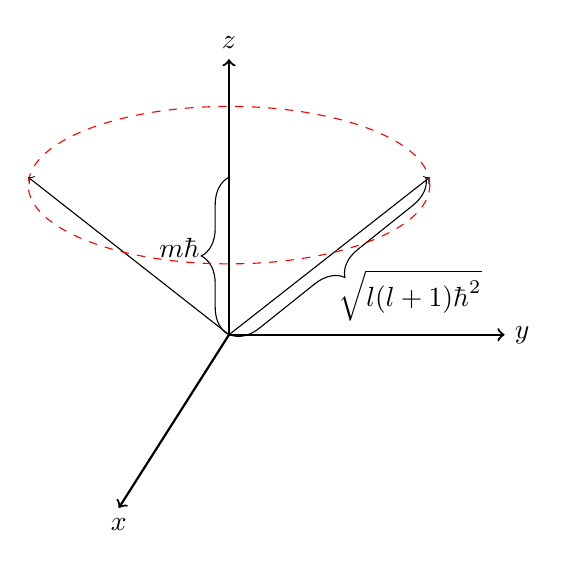
\begin{tikzpicture}[decoration={brace,amplitude=10pt}]
\draw[->,thick] (0,0) -- (0,3.5) node[above] {$z$};
\draw[->,thick] (0,0) -- (3.5,0) node[right] {$y$};
\draw[->,thick] (0,0) -- (-1.4,-2.2) node[below] {$x$};
\draw[decorate] (0,0) --  (0,2);
\node[left] at (-0.25,1.1) {$m\hbar$};
%\draw[dashed] (0,2) -- (2.5,2);
\draw[->] (0,0) -- (2.55,2);
\draw[decorate] (2.5,2) -- (0,0);
\node at (2.3,0.5) {$\sqrt{l(l+1)\hbar^2}$};
\draw[->] (0,0) -- (-2.55,2);
%\draw[decorate] (0,0) -- (-2.5,2);
%\node[rotate=-38.6] at (-1.7,0.5) {$\sqrt{l(l+1)\hbar^2}$};
\draw[dashed,red] (0,1.9) ellipse (2.55 and 1);
\end{tikzpicture}\\
\captionof{figure}{Intuitives Model wobei die rote Kreisbahn den Abstand $\sqrt{l(l+1)\hbar^2}$ zum Mittelpunkt hat und parallel zur $x,y$-Achse liegt}
\end{minipage}%
\begin{minipage}[h]{0.55\textwidth}
	\begin{align*}
	| \vec{l} | &= \sqrt{ l ( l+1) \hbar^2} \\
	l_z &= m \hbar \\
	\langle l_x \rangle &= 0 \\
	\langle l_y \rangle &= 0
	\end{align*}
\end{minipage}%
\newpage
\textbf{Beispiel:}\\
$ l=2 $, $ m = -2, -1, 0, 1, 2 $\\[5pt]
$ \Rightarrow |\vec{l}| = \sqrt{6}\hbar $

%t6
\begin{minipage}[ht]{0.5\textwidth}
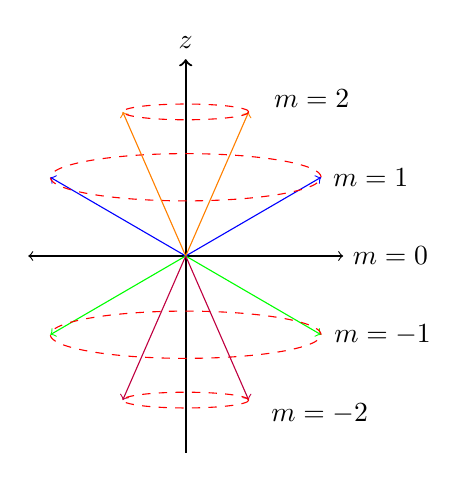
\begin{tikzpicture}[decoration={brace,amplitude=10pt}]
\draw[->,thick] (0,-2.5) -- (0,2.5) node[above] {$z$};
%\centerarc[](0,0)(0:360:2);
\draw[->] (0,0) -- (2,0);
\draw[->] (0,0) -- (-2,0);
\node at (2.6,0) {$m=0$};

\draw[blue,->] (0,0) -- (1.72,1);
\draw[blue,->] (0,0) -- (-1.72,1);
\draw[dashed,red] (0,1) ellipse (1.72 and 0.3);
\node at (1.6,2) {$m=2$};
	
\draw[orange,->] (0,0) -- (0.8,1.83);
\draw[orange,->] (0,0) -- (-0.8,1.83);
\draw[dashed,red] (0,1.83) ellipse (0.8 and 0.1);
\node at (2.35,1) {$m=1$};
	
\draw[green,->] (0,0) -- (1.72,-1);
\draw[green,->] (0,0) -- (-1.72,-1);
\draw[dashed,red] (0,-1) ellipse (1.72 and 0.3);
\node at (2.5,-1) {$m=-1$};
	
\draw[purple,->] (0,0) -- (0.8,-1.83);
\draw[purple,->] (0,0) -- (-0.8,-1.83);
\draw[dashed,red] (0,-1.83) ellipse (0.8 and 0.1);
\node at (1.7,-2) {$m=-2$};
\end{tikzpicture}
\centering
\captionof{figure}{Präzession um die $ z $-Achse hängt von der Quantenzahl $ m $ ab.}
\end{minipage}%
%t7
\begin{minipage}[t]{0.5\textwidth}
\begin{tikzpicture}
\draw[->] (0,0) -- (0,2) node[above] {$\vec{B}$};
\draw[->] (0,0) -- (2,0) node[right] {$\vec{l}$};
\draw[->] (0,0) -- (1.3,1.2) node[right] {$\vec{l}$};
\draw[->] (0,0) -- (-0.8,1.6);
\end{tikzpicture}
\centering
\captionof{figure}{Zeeman Effekt}
\end{minipage}%

\section{Experimente: Wasserstoffatom Spektrum}

Präsentation auf Folien: Wasserstoffatom\\[5pt]
\folie{Balmer Series: Wasserstoffatom}\\
Es gibt verschiedene Zustände im Atom. Man misst das Licht, dass von diesem Atom emittiert wird mit einem Spektrometer. Man erhält Spektrallinien (zunächst einmal die \textbf{Balmer Serie}). Beispielsweise die schwarzen Absorptionslinien im Sonnenspektrum oder diskrete Emissionslinien im Wasserstoffspektrum. Die Linien befinden sich im sichtbaren Spektrum und im nahen UV Die Position der Linien führte auf die \textbf{Balmer Gleichung}:
\begin{equation*}
\lambda = B \left(\frac{m^2}{m^2 - 4}\right)
\end{equation*}
\folie{Lyman Series: Wasserstoffatom}
Später wurde dann die \textbf{Lyman Serie}. Diese Linien sind eher im UV Bereich zu finden. Auch für ihre Positionen konnte eine Gleichung aufgestellt werden.
\begin{equation*}
\lambda = \frac{1}{R_H} \left(\frac{m^2}{m^2 - 1}\right)
\end{equation*}
\folie{Bohrsches Atommodell}\\
Im Bohrschen Atommodell geht man von festen Umlaufbahnen der Elektronen um den Atomkern aus. Bohr hat eine Quantisierung des Drehimpulses eingeführt als die Stationären Zustände der De-Broglie Wellenlänge der Elektronen.\\
Mit der Quantisierung der Umlaufbahnen kommt man zu Schlussfolgerung, dass die Energie der Elektronen nicht beliebig sondern diskret ist. Durch die Energie der emittierten Photonen konnte die \textbf{Rydberg-Formel} aufgestellt werden, die die Wellenlängen der Balmer- und der Lyman-Serie beschreibt.
\begin{equation*}
\lambda = \frac{h c}{R_{y}} \left(\frac{m^2 n^2}{m^2 - n^2}\right)
\end{equation*}
\folie{Rydberg Saal in Lund}\\
Bild der Originalen Gleichung von Rydman an einer Wand verewigt.\\[10pt]
Wie man an der allgemeineren Rydberg-Formel kann man erkennen, dass die Balmer Serie ein Spezialfall für $ n = 2 $ und die Lyman-Serie ein Spezialfall für $ n = 1 $ ist.\\
\folie{Übergänge zwischen stationären Zuständen}\\
Alle weiteren bekannten Serien wie: Balmer, Lyman, Paschen, Brackett, und Pfund.

\subsection*{Morgen}

\begin{itemize}
	\item Energie des Wasserstoffatoms
	\item Korrespondenzprinzip: ($ \vec{r} \to \vec{r} $, $ \vec{p} \to - i \hbar \vabla $) Zeitunabhängige Schrödingergleichung
	\item Energiezustände und Eigenwerte
	\item Drehimpulsoperator $ \vec{l} $ und Kugelflächenfunktionen $ \mathcal{Y}_{l,m}(\theta, \varphi) $
\end{itemize}

% 2.05.19

\subsection*{Lach und Sachgeschichten, heute mit:}
\begin{itemize}
	\item Wasserstoffatom mit Schrödingergleichung
	\begin{itemize}
		\item Wellenfunktion (Quantenzahlen)
		\item Energieniveaus (Entartung)
	\end{itemize}
	\item Spektroskopie
	\begin{itemize}
		\item Wasserstoffatom
		\item Spektrometer
		\item Balmar-Serie
	\end{itemize}
	\item Zeeman Effekt
	\item und natürlich mit der Maus
\end{itemize}
%T1
\hft\\
Energie des Wasserstoffatoms:
$$E=\frac{p_k^2}{2M}+\frac{p_e}{2m_e}+V(r)=\ub{\frac{p_k^2}{2M}}_\text{Kern}+\ub{\frac{p_e^2}{2m_e}}_\text{Elektron}-\ub{\frac{e^2}{4\pi\epsilon_0}\frac{1}{r}}_\text{Coulomb}$$
$$\vec{R_k}=\vec{R_{cM}}+\vec{r_k}$$
$$\vec{R_1}=\vec{R_{cM}}+\vec{r_1}$$
Energie des Wasserstoffatoms im Schwerpunktsystem:
$$E=\frac{p^2_{cM}}{2M_{tot}}+\frac{p^2}{2\mu}-\frac{e^2}{4\pi\epsilon_0}\frac{1}{r}$$
\begin{itemize}
	\item $M_{tot}=M+m$
	\item $\vec{m_{cM}}=(m_e+M)\vec{v_{cM}}$ Impuls des Schwerpunktes
	\item $\mu=\frac{m_eM}{m_e+M}=\frac{m_e}{\frac{m_e}{M}+1}\approx m_e$ Reduzierte Masse mit $m_e \ll M$
	\item $\vec{p}=\frac{1}{M+m_e}[m_e\vec{p}_k-M\vec{p_1}]$ relatives Moment
\end{itemize}

Hamiltonoperator lässt sich in ähnlicher Weise auseinander ziehen.
$$E_{cM}=\frac{p_{cm}^2}{2M_{tot}} \qquad \qquad E_0=\frac{p^2}{2\mu}-\frac{e^2}{4\pi \epsilon_0}\frac{1}{r}$$
$$E\Rightarrow \hat{H}\equiv H$$
$$H=H_{cM}+H_0$$
\begin{align*}
&H_{cm}=\frac{p^2_{cM}}{2M_{tot}}\overset{*}{=}-\frac{\hbar^2}{2M_{tot}}\nabla^2_{cM}\\
&H_0=\frac{p^2}{2\mu}-\frac{e^2}{4\pi \epsilon_0}\frac{1}{r}=-\frac{\hbar^2}{2\mu}\nabla^2-\frac{e^2}{4\pi \epsilon_0}\frac{1}{r}
\end{align*}
$(*)$ $p_{cM}$ als Operator da $H$ ein Operator ist: $ p_{cM}=-i\hbar \nabla_{cM} $
Eigenzustände für $H_{cM}$ und $H_0$:\\
\ \\
$H_{cm}$ ist der Hamilton für ein freies Teilchen
$$\overset{\text{Schrödinger GL}}{\Rightarrow} H_{cM}*\Psi_{cM}=E_{cM}\Psi_{cM}\Rightarrow\frac{-\hbar^2}{2M_{tot}}\nabla^2\Psi_{cM}=E_{cM}\Psi_{cM}$$
Für die Wellengleichung eines freien Teilchens gilt:
$$\Psi_{cM}(\vec{R_{cM}})=Ce^{i(\vec{p_{cM}}\vec{R_{cM}})}\frac{1}{\hbar}$$
$$\Rightarrow -\frac{\hbar^2}{2M_{tot}}\nabla^2\Psi_{cM}=-\frac{\cancel{\hbar^2}}{2M_{tot}}\frac{-\vec{p_{cM}^2}}{\cancel{\hbar^2}}\cancel{\Psi_{cM}}=E_{cM}\cancel{\Psi_{cM}}$$
$$\Rightarrow \frac{\vec{p}^2_{cM}}{2M_{tot}}=E_{cM}$$
Schwerpunkt:
$$H_0=\frac{p^2}{2\mu}-\frac{e^2}{4\pi\epsilon_0}\frac{1}{r}\overset{\mu=m_e}{\approx}\frac{p^2}{2m_e}-\frac{e^2}{4\pi\epsilon_0}$$
Relative Bewegung des Wasserstoffs:
$$\Rightarrow \rmbox{-\frac{\hbar}{2m_e}\nabla^2\Psi(\vec{r})-\frac{e^2}{4\pi\epsilon_0}\frac{1}{r}\Psi(\vec{r})=E_0\Psi(\vec{r})}$$
Lösen der Gleichung mit Kugelkoordinaten:
$$\nabla^2=\frac{1}{r^2}\frac{\partial}{\partial r}(r^2\frac{\partial}{\partial r})-\frac{l^2}{\hbar^2r^2}$$
$l^2=$ Drehimpulsoperator deshalb verwenden wir Kugelflächenfunktionen da wir dort diesen auch vorfinden.\\
Aufspalten der Wellenfunktion in einen Radial und einen Winkelanteil:
$$\Psi(r)=\ub{R_{E_0,l}(r)}_{\text{Radialteil}}\text{ }\ub{\ssf_{l,m}(\theta,\phi)}_{\text{Winkelanteil}}$$
$$\Rightarrow -\frac{\hbar^2}{2m_e}\left[\frac{1}{r^2}\frac{\partial}{\partial r}(r^2\frac{\partial}{\partial r})-\frac{l(l+1)\hbar^2}{\hbar^2r^2}\right]R_{E_0,l}(r)-\frac{e^2}{4\pi\epsilon_0}\frac{1}{r}R_{E_0,l}(r)=E_0R_{E_0,l}(r)$$
$$l^2\ssf_{l,m}(\theta,\phi)=l(l+1)\hbar^2\ssf_{l,m}(\theta\phi)$$
$$U_{E_0,l}(r)=rR{E_0,l}(r)$$
\begin{equation}
\frac{d^2U_{E_0,l}(r)}{dr^2}+\frac{2m_e}{\hbar}\left[E_0-V_{eff}(r)\right]U_{E_0,l}(r)=0
\end{equation}
$$V_{eff}(r)=\ub{-\frac{l^2}{4\pi\epsilon_0}\frac{1}{r}}_{\text{Coulomb Potential}}+\ub{\frac{l(l+1)\hbar^2}{2m_er^2}}{\text{Zentrifugalpotential}}$$
\folie{Zentrifugalpotential}\\
Durch lösen von (1.1) erhält man die Hauptquantenzahlen $n$\\
$$\Psi_{l,n,m}(r)=R_{n,l}(r)\ssf_{l,m}(\theta,\phi)$$
Dies sind die drei Quantenzahlen die die Wellenfunktion eines Wasserstoffatoms beschreiben.
\begin{itemize}
\item $n=1,2,3,4,...$
\item $0\leq l \leq (n-1)$
\item $-l\leq m \leq l$
\end{itemize}
\subsection*{Beispiel}
$$n=2\Rightarrow l=0 \rightarrow m=0$$
$$\Rightarrow l=1 \rightarrow m=1,m=0,m=-1$$
Energie hängt im Wasserstoffatom nur von der Hauptquantenzahl ab, im Gegensatz zur Wellenfunktion die von drei abhängig ist.\\
$$E_n=-\frac{1}{2n^2}\frac{e^2}{4\pi\epsilon_0}\frac{m_e}{\hbar^2}$$
Radialer Anteil der Wellenfunktion mit $n=1\Rightarrow l=0$\\
$$R_{10}=2(\frac{1}{a_0})^{\frac{3}{2}}e^{-\frac{r}{a_0}} \qquad \qquad \ub{a_0=\frac{4\pi \epsilon_0 \hbar^2}{m_el^2}}_{\text{Bohrradius (erste Umlaufbahn)}}$$
\folie{Radialer Anteil der Wellenfunktion: $R_{n,l}(r)$}

\begin{equation*}
\left|\psi_{nkm}(\vec{r})\right|^2  \quad \Rightarrow \quad r^2 \dd r \sin \theta \dd \theta \dd \varphi
\end{equation*}
\begin{align*}
\int \left|\psi_{nlm}(\vec{r})\right|^2 \dd \vec{r} &= \int_{r_0}^{r_1} \dd r \int_{\Omega} \sin \theta \dd \theta \dd \varphi \left|\psi_{nlm}(\vec{r})\right|^2 \\
&= \int_{r_0}^{r_1} r^2 \dd r \int_{\Omega} \sin \theta \dd \theta \dd \varphi \left|R_{nl}(\vec{r})\right|^2 \cdot \left|\mathcal{Y}_{lm}(\theta, \varphi)\right|^2 \\
&= \int_{r_0}^{r_1} r^2 \left|R_{nl}(\vec{r})\right|^2  \dd r \ub{\int_{\Omega} \sin \theta \left|\mathcal{Y}_{lm}(\theta, \varphi)\right|^2 \dd \theta \dd \varphi}_{\Omega = 4 \pi} \\
&= \int_{r_0}^{r_1} r^2 \left|R_{nl}(\vec{r})\right|^2 \dd r
\end{align*}

\subsection{Spektrometer}

%T2
\hft
\folie{Spektrometer}

NIST Database für Spektrallinien von Atomen und Molekülen.\\ \texttt{https://www.nist.gov/pml/atomic-spectra-database} und\\ \verb|https://physics.nist.gov/PhysRefData/ASD/lines_form.html|.\\[10pt]
\noindent
Balmer Linie
\begin{align*}
n = 3 \quad &\Rightarrow \quad n = 2 ! \\
n = 4 \quad &\Rightarrow \quad n = 2 ! \\
n = 5 \quad &\Rightarrow \quad n = 2 !? \\
n = 6 \quad &\Rightarrow \quad n = 2 !?? \\
\end{align*}
\folie{Transmission  von $ SiO_2 $ bei verschiedenen Wellenlängen}\\
\folie{Extreme ultraviolet (XUV) Spektrometer}

% 3.05.19

\subsection*{Programm Heute}

\begin{itemize}
	\item Wasserstoffatom: Energie Entartung
	\item Normaler Zeeman Effekt $ \quad $ Magnetfeld $ \vec{B} $
	\item Stern-Gerlach Experiment $ \ \Rightarrow \ $ Spin $ \vec{s} $
	\item Spin $ \vec{s} $
	\item Zusammenfassung zweier Drehimpulsen $ \vec{l} $, $ \vec{s} $ $ \ \Rightarrow \ $ $ \vec{l} + \vec{s} $
	\item Feinstruktur der Energie des Wasserstoffatoms
\end{itemize}

\subsection{Energie; Entartung}

\begin{equation*}
\rmbox{E_n = - \frac{1}{2 n^2} \left(\frac{e^2}{4 \pi \epsilon_0}\right) \frac{m_e}{\hbar^2} }
\end{equation*}
\begin{equation*}
n = 1 \qquad l = 0 \qquad m = 0 \quad \Rightarrow \quad 1 \qquad 1 s
\end{equation*}

\hfw

% hier für n=2 und n = 3 von Damians Aufschrieb in Arrays packen



\noindent
Entartungsgrad
\begin{equation*}
K = \sum_{l=0}^{n-1} (2l + 1) = n^2
\end{equation*}
Radialanteil der Wellenfunktionen
\begin{equation*}
n = 1 \qquad l = 0 \qquad R_{10}(r) = 2 \left(\frac{1}{a_0}\right)^{\nicefrac{3}{2}} e^{-\nicefrac{r}{a_0}}
\end{equation*}
\begin{equation*}
n = 2 \qquad l = 0 \qquad R_{20}(r) = 2 \left(\frac{1}{a_0}\right)^{\nicefrac{3}{2}} \left(1 - \frac{r}{2  a_0}\right) e^{-\nicefrac{r}{2 a_0}}
\end{equation*}
\begin{equation*}
n = 2 \qquad l = 1 \qquad R_{21}(r) = \frac{1}{\sqrt{3}} \left(\frac{1}{2 a_0}\right)^{\nicefrac{3}{2}} \frac{r}{a_0} e^{-\nicefrac{r}{2 a_0}}
\end{equation*}

\subsection{Zeeman Effekt}

\subsubsection{Klassisches Modell:}

%T1 
\hft

\noindent
\textbf{Drehimpuls} $ \vec{l} = \vec{r} \times \vec{p} $\\
\textbf{Strom} $ I = \frac{-e}{T} = -e \frac{v}{2 \pi R} $\\
\textbf{Magnetisches Moment}$ \vec{p}_m $
\begin{equation*}
\vec{p}_m = I \cdot A \cdot \vec{u}_n = I \pi R^2 \cdot \vec{u}_n = - \frac{e v}{2 \cancel{\pi} \cancel{R}} \cancel{\pi} R^{\cancel{2}} \vec{u}_n = - \frac{e v R \vec{u}_n}{2}
\end{equation*}
\begin{equation*}
\left\{ \begin{array}{l}
\vec{p}_m = - \frac{e v R \vec{u}n}{2} \\[5pt] \vec{l} = \vec{r} \times \vec{p} = m_2 v R \vec{u}_n
\end{array} \right.
\end{equation*}
\begin{equation*}
\vec{p}_m = - \frac{e}{2 m_e} m_e v R \vec{u_n = - \frac{e}{2 m_e}}  \cdot \vec{l} = - \frac{e \hbar}{2 m_e \hbar} \vec{l} = - \mu_{B} \frac{\vec{l}}{\hbar}
\end{equation*}
\begin{equation*}
\mu_B = \frac{e \hbar}{2 m_e} = 9{,}27 \cdot 10^{-24} \, \frac{\tx{J}}{\tx{T}} \qquad \tx{\textbf{Bohrsches Magneton}}
\end{equation*}
\textbf{Elektrisches Feld}
\begin{equation*}
E = - \vec{p}_{el} \cdot \vec{E}
\end{equation*}
\textbf{Magnetisches Feld}
\begin{equation*}
E = - \vec{p}_{m} \cdot \vec{B} \quad \Rightarrow \quad E = \mu_B \frac{\vec{l}}{\hbar} \cdot \vec{B} = \mu_B \frac{l_z}{\hbar} \cdot B
\end{equation*}
\begin{equation*}
\vec{B} = B \vec{u}_z
\end{equation*}
Damit erhalten wir:
\begin{equation*}
\rmbox{E = \mu_B \frac{1}{\hbar} \cdot B l_z}
\end{equation*}
mit $ l_z = m \hbar $ führt dieser Zusammenhang zu:
\begin{equation*}
E m = \mu_B \frac{1}{\cancel{\hbar}} B m \cancel{\hbar} = m \mu_B \cdot B
\end{equation*}

%T2
\hft

\noindent
Die Differenz der Entarteten Energieniveaus ist $ \mu_B B $.\\[10pt]
\noindent
\textbf{Hamilton Operator}
\begin{equation*}
\hat{\ham}_0 = \ham_0 \qquad \tx{Wasserstoffatom}
\end{equation*}
\begin{equation*}
\hat{\ham} = \ham = \ham_0 + \ham_B = \ham_0 + \mu_B \frac{1}{\hbar} B l_z
\end{equation*}
Das $ \ham_B $ stammt aus der Wechselwirkung zwischen Wasserstoffatom und $ \vec{B} $-Feld.\\[5pt]
Wir haben gesehen, dass die Operatoren $ l^2 $ und $ l_z $ vertauschen.
\begin{equation*}
\tx{Wasserstoffatom} \qquad \left[l^2 , l_z\right] = 0 \quad \ssf_{lm}(\theta, \varphi)
\end{equation*}
$$ \left\{\ham_0; l^2, l_z\right\} \Rightarrow \psi_{nlm}(\vec{r}) $$
\begin{align*}
\ham_0 \psi_{nlm}(\vec{r}) &= E_n \quad \psi_{nlm}(\vec{r})\\
l^2 \psi_{nlm}(\vec{r}) &= l(l+1) \hbar^2 \ \ \psi_{nlm}(\vec{r})\\
l_z \psi_{nlm}(\vec{r}) &= m \hbar \quad \psi_{nlm}(\vec{r})
\end{align*}
$ \left[\ham_0 \ham_B\right] = 0 $
\begin{equation*}
\ham_B = \frac{\mu_B}{\hbar} B l_z \qquad \ham_{B} | \psi_{nlm}(\vec{r}) \rangle = \frac{\mu_B B}{\hbar} l_z | \psi_{nlm}(\vec{r}) \rangle = \frac{\mu_B B}{\cancel{\hbar}} \cdot m \cancel{\hbar} | \psi_{nlm}(\vec{r})
\end{equation*}
\begin{align*}
\langle \psi_{nlm}(\vec{r}) | \ham_B | \psi_{nlm}(\vec{r}) \rangle = \langle \psi_{nlm}(\vec{r}) | \mu_B B m | \psi_{nlm}(\vec{r}) \rangle = \mu_B B m \langle \psi_{nlm}(\vec{r}) | \psi_{nlm}(\vec{r}) \rangle = \rmbox{\mu_B B m}
\end{align*}

\subsection{Stern-Gerlach Experiment}

\begin{equation*}
Ag = \ub{\left[Kr\right] 4 d^{10}}_{\tx{volle Schale}} 5 s^{1}
\end{equation*}

%T3
\hft

\noindent
$ \Rightarrow $ Wasserstoffähnlich !\\[5pt]
s Zustand $ l=0 \Rightarrow m = 0 $
\begin{equation*}
\vec{F} = - \vabla E_m = \vec{p}_m \cdot \vabla \vec{B}
\end{equation*}
Dieses Modell beschreibt die experimentelle Beobachtungen nicht ausreichend. Daher wurde die Hypothese aufgestellt, dass das Elektron einen weiteren Freiheitsgrad besitzt: den \textbf{Spin}.

\subsection{Spin}

\begin{equation*}
\vec{\mu}_s = - g_s \frac{\mu_B}{\hbar} \vec{s} \qquad \tx{Spinimpuls}
\end{equation*}
\begin{equation*}
\vec{p}_m = \vec{\mu} e = - \frac{\mu_B}{\hbar} \vec{l} \qquad \tx{Bahndrehimpuls}
\end{equation*}
Hierbei ist $ g_s $ der Land\'e Faktor.\\[5pt]
Da wir festgestellt haben, dass bei bekanntem $ l $, $ m $ nur die ganzzahligen Werte zwischen $ -l $ und $ l $ annehmen kann ($-l \le m \le l$).\par
Da wir für den Spin nur 2 Möglichkeiten haben werden diese $ s = + \frac{1}{2} $ sodass:
\begin{equation*}
\Rightarrow \quad m_s = -\frac{1}{2}; +\frac{1}{2}
\end{equation*}
Da wir fordern $ -s \le m_s \le s $



% kommentar von Damian



\noindent
$ \vec{s} $ Spin-Operator: $ \vec{s} $: $ s_x; s_y; s_z $
\begin{align*}
\left[s_x, s_y\right] &= i \hbar s_z \qquad \left[s_x, s_z\right] \neq 0 \qquad \left[s_y, s_z\right] \neq 0 \\
\left[l_x, l_y\right] &= i \hbar l_z \qquad \left[l_x, l_z\right] \neq 0 \qquad \left[l_y, l_z\right] \neq 0
\end{align*}
\begin{align*}
\left[s^2, s_z\right] = \left[s^2, s_x\right] = \left[s^2, s_y\right] = 0 \\
\left[l^2, l_z\right] = \left[l^2, l_x\right] = \left[l^2, l_y\right] = 0
\end{align*}
\begin{align*}
l &\qquad \tx{Drehimpuls Quantenzahl} \qquad -l \le m \le +l\\
s &\qquad \tx{Spinquantenzahl} \qquad \qquad \quad \ \ -s \le m_s \le +s \qquad \overset{\mathclap{\substack{\tx{Elektronen} \\ (\tx{Fermionen})}}}{\Rightarrow} \qquad s = \frac{1}{2}
\end{align*}
\begin{align*}
l^2;l_z \quad \Rightarrow \quad \ssf_{lm}(\theta, \varphi) \qquad l^2 \ssf_{lm}(\theta, \varphi) &= l(l+1) \hbar^2 \ssf_{lm}(\theta, \varphi) \\
l_z \ssf_{lm}(\theta, \varphi) &= m \hbar \ssf_{lm}(\theta, \varphi)
\end{align*}
\begin{align*}
s^2;s_z \quad \Rightarrow \quad \chi_{\nicefrac{1}{2}, m_s} \qquad &s^2 \chi_{\nicefrac{1}{2}, m_s} = s(s+1)\hbar^2 \chi_{\nicefrac{1}{2}, m_s} = \frac{1}{2} \left(\frac{3}{2}\right)\hbar^2 \chi_{\nicefrac{1}{2}, m_s} = \frac{3}{4} \hbar^2 \chi_{\nicefrac{1}{2}, m_s} \\
&b_2 \chi_{\nicefrac{1}{2}, m_s} = m_s \hbar \chi_{\nicefrac{1}{2}, m_s} \\
\end{align*}

\hfw
% oben im align nachtragen |\alpha \rangle und beta und die zwilen dazu


%T3
\hft

\noindent
$ |\alpha \rangle $: $ s^2 | \alpha \rangle = \frac{3}{4} \hbar^2 | \alpha \rangle $ $ \Rightarrow | \vec{s} | = \frac{\sqrt{3}}{2} \hbar $\\
$ s_z | \alpha \rangle = \frac{\hbar}{2} | \alpha \rangle $\\
$ \chi_{\frac{1}{2}, \frac{1}{2}} $\\
spin-up

\noindent
$ | \beta \rangle $: $ s^2 | \beta \rangle = \frac{3}{4} \hbar^2 | \beta \rangle $ $ \Rightarrow |\vec{s}| = \frac{\sqrt{3}}{2} \hbar $\\
$ s_z | \beta \rangle = - \frac{\hbar}{2} | \beta \rangle $\\
$ \chi_{\frac{1}{2}, - -\frac{1}{2}} $\\
spin-down

\subsubsection{Wasserstoffatom}

$ \psi_{nlm}(\vec{r}) $\\[10pt]
Spin: $ \chi_{\frac{1}{2}, m_s} $\\[10pt]
Die gesamte Wellenfunktion des Wasserstoffatoms
\begin{equation*}
\psi(q) = \ub{\psi_{nlm}(\vec{r})}_{\mathclap{\substack{\tx{Räumlicher} \\ \tx{Anteil}}}} \ub{\chi_{\frac{1}{2}, m_s}}_{\mathclap{\substack{\tx{Spin} \\ \tx{Anteil}}}} \qquad \tx{mit} \quad q \equiv (\vec{r}, s)
\end{equation*}
\begin{align*}
\vec{l} \quad & \Rightarrow \quad \vec{p}_m = \vec{\mu}_l = - \frac{\mu_B}{\hbar} \vec{l} \\
\vec{s} \quad & \Rightarrow \quad \vec{\mu}_s = - g_s \frac{\mu_B}{\hbar} \vec{s}
\end{align*}
$ g_s = $ $ g $-Faktor = 2 $ \Rightarrow $ Q.E.D

% 8.05.19

\begin{itemize}
	\item Zusammensetzung $ \verb|l| $ $ \vec{s} $
	\item Feinstruktur des Wasserstoffatoms
\end{itemize}
\begin{equation*}
\vec{j} = \vec{l} + \vec{s} \qquad \tx{Gesamtdrehimpuls}
\end{equation*}
$ j_x; j_y; j_z $
\begin{equation*}
\left[j_x,j_y\right] = \left[l_x + s_x ; l_y + s_y\right] = \ub{\left[l_x, l_y\right]}_{i \hbar l_z} + \left[l_x, s_y\right] + \left[s_x, l_y\right] + \ub{\left[s_x, s_y\right]}_{i \hbar s_z} = i \hbar \left\{l_z + s_z\right\} = i \hbar j_z
\end{equation*}
$ \vec{j} $ Drehimpulsoperator
\begin{equation*}
\begin{array}{cl}
\ub{j^2; j_z} & \\
\ub{l^2; l_z} & \Rightarrow \ssf_{lm}(\theta, \varphi) \\
\ub{s^2; s_z} & \Rightarrow \chi_{\nicefrac{1}{2}}; m_s
\end{array}
\end{equation*}
\begin{align*}
j^2 \to j(j+1)\hbar^2 \quad & \tx{Eigenwerte} \qquad j \tx{ Gesamtdrehimpulsquantenzahl}\\
j_z \to m_j \hbar \quad & \tx{Eigenwerte} \quad -j \le m_j \le j
\end{align*}
Quantenzahlen  $ l $ und $ s $ angegeben $ \Rightarrow  j = ? $\\[5pt]
Wasserstoffatom in einem $ p $-Zustand $ \quad 2p $ $ \begin{array}{cc}
l=1 & \Rightarrow m_l = \pm 1; 0 \\ s= \frac{1}{2} & \Rightarrow m_s = \pm \frac{1}{2}
\end{array} $
\begin{equation*}
\vec{j} = \vec{l} + \vec{s} \qquad \begin{array}{cc}
j_z = l_z + s_z \\
\downarrow \\
m_j = m_l + m_s
\end{array}
\end{equation*}



%Damian zeugs und Tikz
%T1
\hfw
\hft


\noindent
\begin{align*}
m_j = - \frac{3}{2} \Rightarrow j = \frac{3}{2} \quad & \Rightarrow m_j = - \frac{3}{2} ; -\frac{1}{2} ; + \frac{1}{2} ; + \frac{3}{2} \\
m_j = - \frac{1}{2} \Rightarrow j = \frac{1}{2} \quad & \Rightarrow m_j = \phantom{- \frac{3}{2}} - \frac{1}{2} ; + \frac{1}{2}
\end{align*}

\subsubsection*{Zusammensetzung zweier Bahndrehimpulse}

\begin{equation*}
\tx{Helium} \quad \custo{\rightarrow}{\vec{l}_1}{\vec{r}_1} \quad \custo{\rightarrow}{\vec{l}_2}{\vec{r}_2} \qquad \vec{L} = \vec{l}_1 + \vec{l}_2 \qquad L^2 \Rightarrow L(L+1) \hbar^2 \quad L_z \Rightarrow m_L \hbar
\end{equation*}
$ l_1 = 1 \quad \Rightarrow m_{l_1} = \pm 1; 0 $\\
$ l_2 = 2 \quad \Rightarrow m_{l_2} = \pm 2; \pm 1; 0 $
\begin{equation*}
\left[j_x,j_y\right] = \left[l_{1x} + l_{2x} ; l_{1y} + l_{2y}\right] = \ub{\left[l_{1x}, l_{1y}\right]}_{i \hbar l_{1z}} + \left[l_{1x}, l_{2y}\right] + \left[l_{2x}, l_{1y}\right] + \ub{\left[l_{2x}, l_{2y}\right]}_{i \hbar l_{2z}} = i \hbar \left\{l_{1z} + l_{2z}\right\} = i \hbar L_z
\end{equation*}




%T2
\hft



\begin{align*}
(-1;0) &= (m_{l_1} = -1; m_{l_2} = 0 ) \\
(0;-1) &= (m_{l_1} = 0 ; m_{l_2} = -1)
\end{align*}
\begin{align*}
m_L = 3 \Rightarrow L_3 \quad & \Rightarrow m_L = \pm 3; \pm 2; \pm 1; 0 \\
m_L = 2 \Rightarrow L_2 \quad & \Rightarrow m_L = \pm 2; \pm 1; 0 \\
m_L = 1 \Rightarrow L_1 \quad & \Rightarrow m_L = \pm 1; 0
\end{align*}
\begin{align*}
\begin{array}{c}
l_1 = 1 \\ l_2 = 2
\end{array} \quad &\Rightarrow \quad L = 1,2,3  & \qquad \qquad \rmbox{ | l_2 - l_1 | \le L \le l_1 + l_2 } \quad \rmbox{ -L \le m_L \le L } \\
\begin{array}{c}
l = 1 \\ s = \frac{1}{2}
\end{array} \quad &\Rightarrow \quad j = \frac{1}{2} ; \frac{3}{2} & \qquad \qquad \rmbox{ | l - s | \le j \le l + s } \ \ \quad \rmbox{ -j \le m_j \le j }
\end{align*}

\subsubsection*{Vektormodell}

$ \vec{l}; l_z $


%T3
\hft


\begin{align*}
\langle j_x \rangle &= 0 \\
\langle j_x \rangle &= 0
\end{align*}
$ \vec{j} = \vec{l} + \vec{s} $\\[5pt]
$$ l^2; l_z; s^2; s_z $$
\begin{equation*}
\ssf_{lm}(\theta, \varphi) \quad \chi_{\nicefrac{1}{2}, m_s}
\end{equation*}


%T4
\hft

\noindent
$$ j^2; j_z; l^2; s^2 $$
\begin{equation*}
j_z \Rightarrow m_j = \frac{1}{2} \begin{array}{c}
\nearrow \\ \searrow
\end{array} \begin{array}{l}
m_l = 0 ; \ m_s = \frac{1}{2} \\[10pt] m_l = 1; \ m_s = - \frac{1}{2}
\end{array}
\end{equation*}


%T5
\hft


\noindent
1s:  $ m = 1 \quad s \Rightarrow l = 0 \qquad l = 0 \tx{und} b = \frac{1}{2} \Rightarrow j = \frac{1}{2} \qquad \qquad q s_{\nicefrac{1}{2}} $


%Damian
\hfw


\section{Feinstruktur des Wasserstoffatoms}

\begin{equation*}
\begin{array}{l}
\left.\begin{array}{l}
E_{1s} \approx -13{,}6 \, \tx{eV} \\
E_{2s} \approx -3{,}4 \, \tx{eV}
\end{array} \right\} \approx 10 \, \tx{eV} \\
\hspace{6.5pt} E_{3s} \approx -1{,}5 \, \tx{eV} \big\} \approx 2 \, \tx{eV}
\end{array}
\end{equation*}
Feinstruktur $ \approx 10^{-4} \div 10^{-5} \, \tx{eV} $
\begin{itemize}
	\item (Rest-) Ruheenergie des Elektrons
	\item Darwin Term (Compton Wellenlänge)
	\item Spin-Bahn Kopplung
\end{itemize}

\subsection{Restenergie des Elektrons}

\begin{equation*}
E = \sqrt{m_e^2 c^2 + p^2 c^2} \qquad \qquad m_e^2 c^2 \gg p^2 c^2
\end{equation*}
\begin{equation*}
E = m_e c^2 \left[1 + \frac{p^2 c^2}{m_e^2 c^4}\right]^{\nicefrac{1}{2}} \qquad \qquad x = \frac{p^2 c^2}{m_e^2 c^4} \approx 0 \qquad \qquad \left[1 + x\right]^{\nicefrac{1}{2}} = 1 + \frac{1}{2} x - \frac{1}{8}x^2
\end{equation*}
\begin{equation*}
E = m_e c^2 \left\{ 1 + \frac{1}{2} \frac{p^2 c^2}{m_e^2 c^4} - \frac{1}{2} \left(\frac{p^2 c^2}{m_e^2 c^4}\right)^2 \right\} = \custo{\rightarrow}{m_e c^2}{\tx{Verschiebung}} + \custo{\rightarrow}{\frac{p^2}{2 m_e}}{- \frac{\hbar^2 \vabla^2}{2 m_e}} \rmbox{- \frac{1}{8} \frac{p^4}{m_e^3 c^2} }
\end{equation*}
$ \psi_{nlm}(\vec{r}) $
\begin{equation*}
\Delta E_1 = \langle \psi_{nlm}(\vec{r}) | - \frac{1}{8} \frac{p^4}{m_e^3 c^2} | \psi_{nlm}(\vec{r}) \rangle = \int \dd \vec{r} \psi_{nlm}^{*} \left[- \frac{p^4}{m_e^3 c^2}\right] \psi_{nlm}(\vec{r})
\end{equation*}
$ \vec{p} \Rightarrow - i \hbar \vabla $ einsetzen liefert:

\frbox{Korrekturterm}{
\begin{equation*}
\Delta E_1 = - E_n \frac{\alpha^2}{n^2} \left[\frac{3}{4} - \frac{n}{e + \frac{1}{2}}\right]
\end{equation*}}
$ n = $ Hauptquantenzahl\\
$ \alpha = $ Feinstrukturkonstante $ \alpha = \frac{e^2}{4 \pi \epsilon_0 \hbar c} \approx \frac{1}{137} $\\[10pt]
$ n=1, l=0 $ 1s Zustand
\begin{equation*}
\Delta E_1 = - E_{100} \frac{\alpha^2}{1} \left[\frac{3}{4} - \frac{1}{\frac{1}{2}}\right] = -E_{100} \alpha^2 \left(- \frac{5}{4}\right) = \frac{5}{4} \alpha^2 E_{100} \simeq 9 \cdot 10^{-4} \, \tx{eV}
\end{equation*}
\begin{equation*}
E_{100} = E_{nlm} = - 13{,}5 \, \tx{eV}
\end{equation*}

\subsection{Darwin Term (Compton Wellenlänge)}


%T6
\hft


\begin{equation*}
V(r) = -\frac{e^2}{4 \pi \epsilon_0} \frac{1}{r}
\end{equation*}
$ \lambda \nu = c \quad \Rightarrow \quad \nu = \frac{c}{\lambda} $
\begin{equation*}
\left. \begin{array}{l}
E = m_e c^2  \\
E = h\nu = h \frac{c}{\lambda}
\end{array} \right\} \Rightarrow m_e c^{\cancel{2}} = h \frac{\cancel{c}}{\lambda} \quad \Rightarrow \quad \lambda = \frac{h}{m_e c}
\end{equation*}
\begin{equation*}
V(r) = -\frac{e^2}{4 \pi \epsilon_0} \frac{1}{r}
\end{equation*}
\begin{equation*}
\Rightarrow \quad V_{\tx{eff}}(r) = \int \dd \vec{r}' \frac{e}{4 \pi \epsilon | \vec{r} - \vec{r}'|} \rho (\vec{r} + \vec{r}')
\end{equation*}
Im folgenden soll $ \lambda_{C} $ die reduzierte Compton-Wellenlänge also $ \frac{\lambda_C}{2 \pi} $ bezeichnen.


%T7
\hft


\noindent
\begin{equation*}
\lambda_{C} = \frac{h}{m_e c} \frac{1}{2 \pi}
\end{equation*}
\begin{equation*}
\rho(\vec{r} + \vec{r}') = \casess{- \frac{e}{\left(\frac{4}{3} \pi \lambda^3 c \right)}}{| \vec{r}'| < \lambda_C}{0}{| \vec{r}'| > \lambda_C}
\end{equation*}
\begin{equation*}
V_{\tx{eff}} (\vec{r}) = V(r) + \frac{\pi}{2} \lambda^2 c \frac{e^2}{4 \pi \epsilon_0} \custo{\rightarrow}{\delta(\vec{r})}{\tx{Dirac Delta}}
\end{equation*}
\begin{equation*}
\Delta E_2 = \frac{\pi}{2} \lambda^2 c \frac{e^2}{4 \pi \epsilon_0} \quad \langle \psi_{nlm}(\vec{r}) | \delta(\vec{r}) | \psi_{nlm}(\vec{r}) \rangle
\end{equation*}
$ l=0 $ $ s $-Zustände
\begin{equation*}
\Delta E_2 = - E_n \frac{\alpha^2}{n}
\end{equation*}
mit $ n $ der Hauptquantenzahl
\begin{equation*}
\frac{\Delta E_2}{E_{100}} = - \alpha^2 = - 5{,}3 \cdot 10^{-5}
\end{equation*}

\subsection*{Programm Heute}
\begin{itemize}
\item Spin-Bahn Kopplung
\item Feinstruktur des Wasserstoffs
\item Zeeman Effekt $\begin{array}{l}\rightarrow \textrm{Anomaler Zeeman Effekt} \\ \rightarrow \textrm{Normaler Zeeman Effekt} \\ \rightarrow \textrm{Paschen-Back Effekt}\end{array}$ % OwO
\item Spin Bahn Kopplung
\end{itemize}
\begin{minipage}{0.4\textwidth}
\begin{align*}
L &= 1:2_{} & 2p & \rightarrow \begin{matrix}2p_{\nicefrac{1}{2}} \\ 2p_{\nicefrac{3}{2}}\end{matrix} \\
& \bar{L} \Rightarrow \vec{\mu}_C = -\frac{\mu_B}{\hbar}\vec{L} \\
& \bar{s} \Rightarrow \vec{\mu}_s = -g_s \frac{\mu_B}{\hbar}\vec{s}
\end{align*}
\end{minipage}
\begin{minipage}{0.4\textwidth}
%T1
\hft
\end{minipage}

\begin{minipage}{0.4\textwidth}
Bezugssystem des Elektrons:

%T2
\hft

\end{minipage}
\begin{minipage}{0.4\textwidth}
Bio Savart Gesetz:
\begin{align*}
\mathrm{d}\bar{B} &= \frac{\mu_0}{4\pi} I \frac{\mathrm{d}I\times\Delta\vec{r}}{|\Delta r|^3} & \Rightarrow B &= \frac{\mu_0I}{2r} \\
I &= \frac{e}{T} \frac{ev_K}{2\pi r_K} & \rightarrow B&= \frac{\mu_0}{2r} \frac{ev_K}{2\pi r_K} = \frac{\mu_0 e v_K r_K}{4 \pi r_K^3}
\end{align*}
\end{minipage}
\\
\\
\begin{equation*}
B = \frac{\mu_0 e v_K r_K}{4\pi r_K^3} \Rightarrow \vec{B} = \frac{\mu_0 e }{4 \pi r_K^3} = \frac{\mu_0 e}{4 \pi r_K^3 m_e}\vec{r}_K \times m_e \vec{v}_K
\end{equation*}

\[
B = \frac{\mu_0 e}{4 \pi r^3 m_e} (\vec{r} \times m_e \vec{v})\underbrace{\frac{1}{2}}_{\mathclap{\substack{\textrm{Thomas Faktor aus} \\ \textrm{Lorenz Transformation}}}}
\]

\begin{align*}
\rmbox{ B = \frac{\mu_0 e }{8 \pi r^3 m_e}\vec{L}} & & \vec{L} &= \vec{r} \times \m_e \vec{v} = \vec{r}\times\vec{p}
\end{align*}

\[
E = -\underbrace{\vec{\mu}_s}_{{\substack{\textrm{Magnetisches} \\ \textrm{Dipolmoment}}}} \cdot \underbrace{\vec{B}_r}_{{\substack{\textrm{"au\ss eres} \\ \textrm{ Magnetfeld}}}} = -\underbrace{(-g_s \frac{\mu_B}{\hbar} \vec{s})}_{\mu_s} \cdot \underbrace{\frac{\mu_0 e}{8 \pi r^3 m_e} \vec{L}}_{B} = \underbrace{g_s \mu_B \frac{\mu_0e}{8 \pi r^3 m_e}\frac{1}{\hbar}\vec{s}\vec{L}}_{\mathclap{\textrm{nur abh"angig von }r,\ \vec{s},\ \vec{L}}}
\] % I'm so sorry.

\[\textrm{Suchen }\vec{s}\cdot\vec{L}:\ \vec{j} = \vec{L} + \vec{s} \Rightarrow \vec{j}^2 = \vec{L}^2 + \vec{s}^2 + 2\vec{L} \cdot\vec{s} \Leftrightarrow \vec{L} \cdot \vec{s} = \frac{1}{2}(j^2 - L^2 - s^2)\]
Eigenzust"ande: $j^1;\ L^2;\ s^2$ \\
Basen: $\{ L^2;\ L_2;\ s^2;\ s_2\ \underbrace{\rmbox{\{j^2;\ L_2;\ s^2;\ j_2}}_{\textrm{Fokus auf die 2. da dort }j\textrm{ dabei ist.}}$

\[
E = \frac{\mu e^2}{8 \pi r^3 m_2^2}\cdot \vec{s}\cdot \vec{L} = \frac{\mu_0 e^2}{8\pi r^3 m_e^2} \frac{1}{2} [j^2 - L^2 - s^2] \Rightarrow H_{SO} = \textrm{Spin-Bahn Kopplung}
\]

\[
E = \langle H_{SO}\rangle = \frac{\mu_- e^2}{8\pi m_e^2} \frac{1}{2} \left\langle njLsj_z\Bigg|\frac{1}{r^3}Lj^2 - L^2 - s^2 \Bigg| njLsj_2\right\rangle
\]
% Quantenzahlen unseres Systems in neuer Basis davor |n, L, m\langle;|nLmm_s\rangle diesmal aber nicht benutzbar. (Da wir immer die Eigenzust"ande w"ahlen m"ussen.)

\[
E = \langle H_{SO}\rangle = \underbrace{\frac{\mu_0 e^2}{8\pi m_e^2} \frac{1}{2} \frac{1}{r^3nL}}_{\textrm{radial Anteil}} \underbrace{\langle jLsj_z | Lj^2-L^2-s^2 | jLsj_z\rangle}_{\textrm{Winkelanteil}}
\]

\[
\left\langle\nicefrac{1}{r^3}\right\rangle = \left\langle nL | \nicefrac{1}{r^3} |nL\right\rangle = \frac{1}{r^3m_e}
\]

\[
E = \langle H_{SO}\rangle = \frac{\mu_0 e^2}{8\pi m_e^2} \frac{1}{2} \frac{1}{r^3m_e}\{j(j+1)\hbar^2 - L(L+1)\hbar^2 - s(s+1)\hbar^2\}
\]

\[
\rmbox{
E = \langle H_{SO} \rangle = \frac{a}{2} [j(j+1) - L(L+1) - s(s+1)]}\qquad a = \frac{\mu_0 e^2}{8\pi m_e^2}\frac{1}{rm_e} \hbar^2
\]

\begin{itemize}
\item 
$j = L-\frac{1}{2}$ \begin{align*} E=\langle H_{SO}\rangle &= \frac{a}{2}[(L-\nicefrac{1}{2})(L+\nicefrac{1}{2}) - L(L+1) - \nicefrac{3}{4}] \\
&=-\frac{a}{2}(L+1)
\end{align*}
\item 
$j = L+\frac{1}{2}$ \begin{align*} E=\langle H_{SO}\rangle &= \frac{a}{2}[(+-\nicefrac{1}{2})(L+\nicefrac{1}{2}) - L(L+1) - \nicefrac{3}{4}] \\
&=\frac{aL}{2}
\end{align*}
\end{itemize}

Aufspaltung der Energie einmal gr"o\ss er einmal kleiner.
%T3
\hft
\[
\frac{\Delta e_3}{E_{210}} = -\frac{\alpha^2}{12} = -4\cdot44\cdot10^{-6}
\]
\[
210 \Rightarrow n=2,\ L=1 \Rightarrow \textrm{2p Zustand} \Rightarrow j=\frac{3}{2}
\]
$\Delta E_1,\ \Delta E_2,\ \Delta E_3$ alle Beschrieben
\frbox{Feinstruktur der Energieniveaus}{
\[\Delta E_\mathrm{FStruktur} = \Delta E_1 + \Delta E_2 + \Delta E_3 = E_m\left[\frac{\alpha^2}{n}\left(\frac{1}{j+\nicefrac{1}{2}} - \frac{3}{4n}\right)\right]\]
}
nur von $n$ und $j$ abh"angig.

%T4
\hft

\hfw

%%%%%%%%%%%%%%%%%%%%%%%%%%%%%%%
% Hier Fehlt etwas von Damian %
%%%%%%%%%%%%%%%%%%%%%%%%%%%%%%%


% 16.05.19

\subsubsection*{Programm Heute:}

\begin{itemize}
	\item Anormaler Zeeman Effekt $ j $
	\item Normaler Zeeman Effekt
	\item Paschen-Back Effekt
	\item Hyperfeinstruktur (Wasserstoffatom): Atomuhr
	\item Lamb Shift
\end{itemize}

\subsection{Normaler Zeeman Effekt}

$ \vec{S} = 0 \quad $ Helium $ \vec{S} = \vec{s}_1 + \vec{s}_2 $ \lcom{Beim Heliumatom gibt es zwei Spins für die beiden Elektronen. Es gibt hier zwei Möglichkeiten: entweder up-up und down-down \textbf{oder} up-down und down-up. Deher gibt es zwei Möglichkeiten für den Gesamtspin.}
\begin{equation*}
\vec{S} \begin{array}{c}
\nearrow \\[5pt] \searrow
\end{array} \ \begin{array}{l}
S = 0 \quad \Rightarrow \tx{Normaler Zeeman Effekt} \\[10pt] S = 1 \quad \Rightarrow \tx{Anormaler Zeeman Effekt}
\end{array}
\end{equation*}
\begin{equation*}
H = H_0 + \frac{\mu_B}{\hbar_0} \vec{L} \cdot \vec{B} \qquad \vec{L} = \vec{l_1} + \vec{l}_2
\end{equation*}
Energie Verschiebung
\begin{equation*}
E_B = \frac{\mu_B}{\hbar_0} \vec{L} \cdot \vec{B} = \frac{\mu_B}{\hbar_0} L_z \cdot B
\end{equation*}
mit $ L_z = m_z \hbar $
\begin{equation*}
\rmbox{E_B = \frac{\mu_B}{\cancel{\hbar_0}} m_z \cancel{\hbar_0} B = \mu_B m_z B } 
\end{equation*}

% lcom von damian

\subsection{Pasch-Bach Effekt}

$ E_{so} \ll E_{B} $
\begin{equation*}
H = H_0 + \frac{\mu_B}{\hbar} \left(\vec{l} + 2 \vec{s}\right) \cdot \vec{B} = H_0 + \frac{\mu_B}{\hbar} \left(l_z + 2 s_z\right) \cdot B
\end{equation*}
Operatoren $ l^2; l_z; s^2, s_z $
\begin{equation*}
\rmbox{ E_B = \frac{\mu_B}{\hbar} \left(m_l \hbar + 2 m_s \hbar \right) \cdot B = \mu_B \left(m_l + 2 m_s\right) \cdot B }
\end{equation*}
Betrachten wir hierzu ein Beispiel:\\[5pt]
Was passiert mit dem $ p $-Zustand wenn wir ein starkes äußeres Magnetfeld anlegen, sodass die Spin-Bahn-Kopplung vernachlässigbar klein wird: $ p $-Zustand $\quad  l=1 \quad s = \frac{1}{2} $\\
%t1: (schon als tabelle gemacht)
\begin{tabular}{c|c|c}
	$ m_l $ & $ m_s $ & $ m_l + 2 m_s $ \\ \hline
	$ -1 $ & $ -\nicefrac{1}{2} $ & $ -2 $ \\
	\color{green!50!black}$ \mathbf{-1} $ & \color{green!50!black}$ +\nicefrac{1}{2} $ & \color{green!50!black}$ \mathbf{0} $ \\
	$ 0 $ & $ -\nicefrac{1}{2} $ & $ -1 $ \\
	$ 0 $ & $ +\nicefrac{1}{2} $ & $ +1 $ \\
	\color{green!50!black}$ \mathbf{1} $ & \color{green!50!black}$ -\nicefrac{1}{2} $ & \color{green!50!black}$ \mathbf{0} $ \\
	$ 1 $ & $ +\nicefrac{1}{2} $ & $ +2 $ \\
\end{tabular}
$ B \neq 0 $

%T2
\hft


\noindent
$ p \dots $ mit $ l=1 \quad s = \frac{1}{2} \quad m_l = 0; \pm 1 \quad m_s = \pm \frac{1}{2} $\\
\folie{Anormaler Zeeman- und Paschen-Bach-Effekt Kombination beider Effekte}\\
\folie{Natrium Energieniveaus} $ \quad [\tx{Na}] = [\tx{NA}] 3 s^1 \ n^{2 s +1} \ L_j $\\
$ n^{2s + 1} L_j  \quad \vec{J} = \vec{L} + \vec{S} $\\
$ s = \frac{1}{2} = S \quad 2 S + 1 = 2 $\\
$ l = 0 = L $\\[5pt]
$ \Rightarrow \vec{J} = L + S = \frac{1}{2} $

\subsection{Hyperfeinstruktur}

$ 10^{-6} \div 10^{-8} \, \tx{eV} $\\
\begin{minipage}{.7\linewidth}
	Drehimpuls des Kerns $ \vec{I} $ (des Protons) Wasserstoff
	\begin{equation*}
	E_{HFS} = - \vec{\mu_I} \cdot \vec{B}_j \qquad \vec{\mu_I} = g_I \frac{\mu_K}{\hbar} \vec{I}
	\end{equation*}
	$ g_I = $ Kern $ \rho $ Faktor\\
	$ \mu_{K} = $ Kernmagneton
\end{minipage}%
\begin{minipage}{.3\linewidth}
	\flushright
	%t3:
	\begin{tikzpicture}[scale=0.75]
		\draw[dashed] (0,0) circle (1.5cm);
		\draw[fill=black] (0,0) circle (1pt) node[anchor=north east] {$ e $};
		\coordinate (e) at (1.5,0);
		\draw[thick, ->] (e) -- ++(0,1) node[anchor=north west] {$ e $};
		\draw[fill=blue, draw=black] (e) circle (2pt);
	\end{tikzpicture}
\end{minipage}%
\begin{equation*}
\mu_{K} = \frac{e}{2 m_p} \hbar = \frac{e}{2 m_e} \hbar \frac{m_e}{m_p} = \mu_B \frac{m_e}{m_p} = \mu_{B} \frac{1}{1836}
\end{equation*}
$ \vec{B}_i \propto - \vec{i} $
\begin{equation*}
E_{HFS} = - \vec{\mu}_I \cdot \vec{B}_{j} = - |\vec{\mu}_j| \cdot B_j \cos(\vec{\mu}_I , \vec{B}_j) = \rmbox{| \vec{\mu}_I| B_j \cos(\vec{I}, \vec{j}) }
\end{equation*}
\begin{equation*}
\cos(\vec{j}, \vec{I}) = \frac{\vec{j} \vec{I}}{|\vec{j}| |\vec{I}|} \quad \Rightarrow \quad \vec{j} \cdot \vec{I}
\end{equation*}
\begin{equation*}
\vec{F} = \vec{I} + \vec{j} = \ \tx{Gesamtdrehimpuls des Atoms} \quad \begin{array}{l}
\vec{I} \Rightarrow \tx{Kern (proton)} \\ \vec{j} \Rightarrow \tx{Elektron}
\end{array}
\end{equation*}
\begin{equation*}
|\vec{F}| = \sqrt{F(F+1)} \hbar \qquad \qquad -f \le m_F \le f
\end{equation*}
\begin{equation*}
\cos(\vec{I}, \vec{j}) = \frac{1}{2} \frac{\left(F^2 - I^2 - j^2\right)}{| \vec{j} | | \vec{I} |} = \frac{1}{2} \frac{\left[F(F+1)\hbar^2 - I(I+1) \hbar^2 - j(j+1) \hbar ^2\right]}{\sqrt{j(j+1)} \hbar \sqrt{I(I+1)} \hbar}
\end{equation*}
\lcom{Ähnliches wurde Vorhin in der Vorlesung bei der Spin-Bahn Kopplung festgestellt.}
\begin{align*}
E_{HFS} = | \vec{\mu}_I | B_j \cos(\vec{I}, j) &= | \vec{\mu}_I | B_j \frac{1}{2} \frac{\left[F(F+1) - I(I+1) - j(j+1)\right]}{\sqrt{j(j+1)} \sqrt{I(I+1)}}\\
&= \rmbox{\frac{A}{2} \left[ F(F+1) - I(I+1) - j(j+1) \right]}
\end{align*}
\begin{equation*}
A = \frac{g_I \mu_K B_j}{\sqrt{j(j+1)}}
\end{equation*}

\subsubsection{Wasserstoff Grundzustand}

\begin{equation*}
\begin{array}{clc}
l=0 \quad s = \frac{1}{2} & \tx{Elektron} & j = \frac{1}{2} \\[5pt]
I = \frac{1}{2} & \tx{Proton} & I = \frac{1}{2}
\end{array} \quad \Rightarrow \vec{F} = \vec{I} + \vec{j} |I-j| \le F \le I+j \begin{array}{c}
\nearrow \\[5pt] \searrow
\end{array} \begin{array}{c}
F = 1 \\[10pt] F = 0
\end{array}
\end{equation*}
\begin{align*}
E_{HFS} (F=0) &= \frac{A}{2} \left[F(F+1) - I(I+1) - j(j+1)\right] = \frac{A}{2} \left[-\frac{1}{2} \left(\frac{1}{2} + 1\right) - \frac{1}{2} \left(1 + \frac{1}{2}\right)\right]\\
&= \frac{A}{2} \left(-\frac{3}{2}\right) = \frac{-3A}{2} \\
E_{HFS} (F=1) &= \frac{A}{2} \left[ 1 \cdot 2 - \frac{3}{4} - \frac{3}{4}\right] = \frac{A}{4}
\end{align*}


%T4 
\hft

\noindent % make left on minipage
$ \Delta E = 5{,}9 \cdot 10^{-6} \, \tx{eV} $\\
$ \nu = 1420 \, \tx{MHz} $\\
$ \lambda = 21 \, \tx{cm} $ (Radioastronomie)

\subsubsection{Wasserstoff erster angeregter Zustand}

\begin{equation*}
\begin{array}{cccc}
l=1 \quad s =\frac{1}{2} & \tx{Elektron} & j = \frac{1}{2}; \frac{3}{2} & \qquad j = \frac{1}{2} ; I = \frac{1}{2} \quad \Rightarrow \quad F = 0,1 \\[10pt]
I = \frac{1}{2} & \tx{Proton} & I=\frac{1}{2} & \qquad j = \frac{3}{2} ; I = \frac{1}{2} \quad \Rightarrow \quad F = 1,2
\end{array}
\end{equation*}
\folie{Atomuhr}\\
\lcom{Die Zeit wird hierbei mit einem Bestimmten Energieübergang definiert. Hierfür ist die Hyperfeinstruktur sehr wichtig.}\\
\folie{Cäsium energy levels}

\subsection{Lamb Shift}

Feinstrukturen $ n; j \qquad \qquad 2 s_{\nicefrac{1}{2}}; 2 p_{\nicefrac{1}{2}} \quad \Rightarrow $ Lamb Shift\\[10pt]
In der Quantenelektrodynamik (QED) gilt:
\begin{equation*}
\Delta E \Delta t \ge \frac{\hbar}{2}
\end{equation*}
\begin{center}
	%t5
	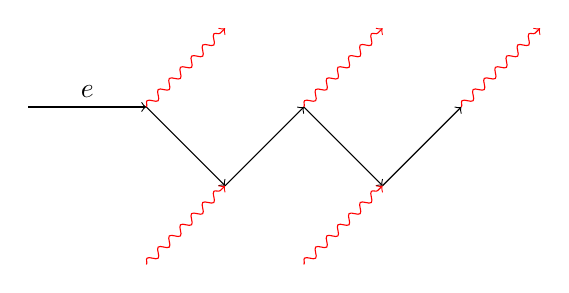
\begin{tikzpicture}
	\draw[->] (-1.5,0) -- node[above] {$ e $} (0,0);
	\draw[->] (0,0) -- ++(1,-1);
	\draw[->] (1,-1) -- ++(1,1);
	\draw[->] (2,0) -- ++(1,-1);
	\draw[->] (3,-1) -- ++(1,1);
	\draw[decorate, decoration={snake, segment length=2mm, amplitude=0.5mm}, red, ->] (0,0) -- (1,1);
	\draw[decorate, decoration={snake, segment length=2mm, amplitude=0.5mm}, red, ->] (0,-2) -- (1,-1);
	\draw[decorate, decoration={snake, segment length=2mm, amplitude=0.5mm}, red, ->] (2,0) -- ++(1,1);
	\draw[decorate, decoration={snake, segment length=2mm, amplitude=0.5mm}, red, ->] (2,-2) -- ++(1,1);
	\draw[decorate, decoration={snake, segment length=2mm, amplitude=0.5mm}, red, ->] (4,0) -- ++(1,1);
	\end{tikzpicture}
\end{center}


Zitterbewegung:
%T6 Zitterbewegung
\hft


\noindent
\begin{equation*}
E_{\tx{pot}} = - \frac{e^2}{4 \pi \epsilon_0} \frac{1}{r} \quad \Rightarrow \quad \langle E_{\tx{pot}} \rangle = - \frac{e^2}{4 \pi \epsilon_0} \left\langle \frac{1}{r + \delta r} \right\rangle
\end{equation*}
\begin{equation*}
\begin{array}{cc}
2s_{\nicefrac{1}{2}} & 2 p_{\nicefrac{1}{2}} \\ l=0 & l=1 \\ \left\langle \frac{1}{r + \delta r} \right\rangle_{2s} & \left\langle \frac{1}{r + \delta r} \right\rangle_{2p} \\ 2 s_{\nicefrac{1}{2}} & 2 p_{\nicefrac{1}{2}} \\
\Delta E = 4{,}3 \cdot 10^{-6} \, \tx{eV} & \Delta E = - 5{,}95 \cdot 10^{-8} \, \tx{eV}
\end{array}
\end{equation*}
\folie{Lamb-Verschiebung: Lamb-Rutherford Experiment}

